\setcounter{chapter}{19}

\chapter{Report Writing: Communicating Data Analysis Results}

{\small \textit{Chapter Preview.} Statistical reports should be
accessible to different types of readers. These reports inform
managers who desire broad overviews in nontechnical language as well
as analysts who require technical details in order to replicate the
study. This chapter summarizes methods of writing and organizing
statistical reports. To illustrate, we will consider a report of
claims from third party automobile insurance.}

\bigskip

\bigskip

\section{Overview}\label{S20:Overview}

The last relationship has been explored, the last parameter has been
estimated, the last forecast has been made, and now you are ready to
share the results of your statistical analysis with the world. The
medium of communication can come in many forms: you may simply
recommend to a client to ``buy low, sell high'' or give an oral
presentation to your peers. Most likely, however, you will need to
summarize your findings in a written report.

Communicating technical information is difficult for a variety of
reasons. First, in most data analyses there is no one ``right''
answer that the author is trying to communicate to the reader. To
establish a ``right'' answer, one only need position the pros and
cons of an issue and weigh their relative merits. In statistical
reports, the author is trying to communicate data features and the
relationship of the data to more general patterns, a much more
complex task. Second, most reports written are directed to a primary
client, or audience. In contrast, statistical reports are often read
by many different readers whose knowledge of statistical concepts
varies extensively; it is important to take into consideration the
characteristics of this heterogeneous readership when judging the
pace and order in which the material is presented. This is
particularly difficult when a writer can only guess whom the
secondary audience may be. Third, authors of statistical reports
need to have a broad and deep knowledge base, including a good
understanding of underlying substantive issues, knowledge of
statistical concepts and language skills. Drawing on these different
skill sets can be challenging. Even for a generally effective
writer, any confusion in the analysis is inevitably reflected in the
report.

\marginparjed{Provide enough details of the study so that the
analysis could be independently replicated with access to the
original data.}

Communication of data analysis results can be a brief oral
recommendation to a client or a 500-page Ph.D. dissertation.
However, a 10- to 20-page report summarizing the main conclusions
and outlining the details of the analysis suffices for most business
purposes. One key aspect of such a report is to provide the reader
with an understanding of the salient features of the data. Enough
details of the study should be provided so that the analysis could
be independently replicated with access to the original data.

\section{Methods for Communicating Data}\label{S20:Methods for Communicating Data}

To allow readers to interpret numerical information effectively,
data should be presented using a combination of words, numbers and
graphs that reveal its complexity. Thus, the creators of data
presentations must draw on background skills from several areas
including:
\begin{itemize} \item an understanding of the underlying substantive
area, \item  a knowledge of the related statistical concepts, \item
an appreciation of design attributes of data presentations and \item
an understanding of the characteristics of the intended audience.
\end{itemize}

\noindent This balanced background is vital if the purpose of the
data presentation is to inform. If the purpose is to enliven the
data (``because data are inherently boring'') or to attract
attention, then the design attributes may take on a more prominent
role. Conversely, some creators with strong quantitative skills take
great pains to simplify data presentations in order to reach a broad
audience. By not using the appropriate design attributes, they
reveal only part of the numerical information and hide the true
story of their data. To quote Albert Einstein, ``You should make
your models as simple as possible, but no simpler.''

This section presents the basic elements and rules for constructing
successful data presentations. To this end, we discuss three modes
of presenting numerical information: (i) within text data, (ii)
tabular data and (iii) data graphics. These three modes are ordered
roughly in the complexity of data that they are designed to present;
from the within text data mode that is most useful for portraying
the simplest types of data, up to the data graphics mode that is
capable of conveying numerical information from extremely large sets
of data.

\subsection*{Within Text Data}

Within text data simply means numerical quantities that are cited
within the usual sentence structure. For example:
\smallskip
\begin{center}The price of Vigoro stock today is \$36.50 per
share, a record high.\end{center}
\smallskip
When presenting data within text, you will have to decide whether to
use figures or spell out a particular number. There are several
guidelines for choosing between figures and words, although
generally for business writing you will use words if this choice
results in a concise statement. Some of the important guidelines
include:
\medskip
\begin{compactenum}[1.]
 \item Spell out whole numbers from one to ninety-nine.
 \item Use figures for fractional numbers.
 \item Spell out round numbers that are approximations.
 \item Spell out numbers that begin a sentence.
 \item Use figures in sentences that contain several numbers.
\end{compactenum}
\medskip
For example:

\medskip

There are forty-three students in my class.

With 0.2267 U.S. dollars, I can buy one Swedish kroner.

There are about forty-three thousand students at this university.

Three thousand, four hundred and fifty-six people voted for me.

Those boys are 3, 4, 6 and 7 years old.

\medskip


Text flows linearly; this makes it difficult for the reader to make
comparisons of data within a sentence. When lists of numbers become
long or important comparisons are to be made, a useful device for
presenting data is the \emph{within text table}, also called the
\emph{semitabular} form. For example:

\bigskip
\boxedjed

For 2005, net premiums by major line of business written by property
and casualty insurers in billions of US dollars, were:

\begin{list}{}{}
 \item Private passenger auto --- 159.57
 \item Homeowners multiple peril --- 53.01
 \item Workers' compensation --- 39.73
 \item Other lines --- 175.09.
\end{list}

(\textit{Source: The Insurance Information Institute Fact Book
2007.})

\end{boxedminipage}

\subsection*{Tables}\index{table}

When the list of numbers is longer, the tabular form, or
\emph{table}, is the preferred choice for presenting data. The basic
elements of a table are identified surrounding Table
\ref{T20:LiquidSumStats}.


\begin{picture}(150,12)
\put (-40,-30){Title \vector(2,0){40}}

\put (-40,-55){Column Headings \vector(2,0){35}}

\put (-40,-120){Stub \vector(2,0){40}}

\put (360,-86){Body}

\put (390,-90){\vector(-2,0){40}}

\put (-40,-168){Rule \vector(2,0){35}}

\end{picture}

\begin{table}[h]
\scalefont{0.9}

\caption{\label{T20:LiquidSumStats} Summary Statistics of Stock
Liquidity Variables}

\begin{tabular}{lrrrrr}
\hline
&  & & Standard &  &  \\
& Mean & Median & deviation & Minimum & Maximum \\
\hline VOLUME & 13.423 & 11.556 & 10.632 &
0.658 & 64.572 \\
AVGT & 5.441 & 4.284 & 3.853 & 0.590 &
20.772 \\
NTRAN & 6436 & 5071 & 5310 & 999 &
36420 \\
PRICE & 38.80 & 34.37 & 21.37 & 9.12 &
122.37 \\
SHARE & 94.7 & 53.8 & 115.1 & 6.7 &
783.1 \\
VALUE & 4.116 & 2.065 & 8.157 & 0.115 &
75.437 \\
DEB\_EQ & 2.697 & 1.105 & 6.509 & 0.185 & 53.628 \\\hline
\multicolumn{6}{l}{\textit{Source: Francis Emory Fitch, Inc.,
Standard \& Poor's Compustat,}}\\
\multicolumn{6}{l}{\textit{~~~and University of Chicago's Center for
Research on Security Prices.}} \\ \hline
\end{tabular}
\scalefont{1.1111}
\end{table}


These are:
\medskip
\begin{compactenum}[1.]
\item \emph{Title.} A short description of the data, placed above or to the side of the
table. For longer documents, provide a table number for easy
reference within the main body of the text. The title may be
supplemented by additional remarks, thus forming a \emph{caption}.
\item \emph{Column Headings}. Brief indications of the material in
the columns.
\item \emph{Stub}. The left hand vertical column. It often provides identifying information
for individual row items.
\item \emph{Body}. The other vertical columns of the table.
\item \emph{Rules}. Lines that separate the table into its various components.
\item \emph{Source}. Provides the origin of the data.
\end{compactenum}
\medskip
As with the semitabular form, tables can be designed to enhance
comparisons between numbers. Unlike the semitabular form, tables are
separate from the main body of the text. Because they are separate,
tables should be self-contained so that the reader can draw
information from the table with little reference to the text. The
title should draw attention to the important features of the table.
The layout should guide the reader's eye and facilitate comparisons.
Table \ref{T20:LiquidSumStats} illustrates the application of some
basic rules for constructing ``user friendly'' tables. These rules
include:
\medskip
\begin{compactenum}[1.]
\item For titles and other headers, STRINGS OF CAPITALS ARE DIFFICULT
TO READ, keep these to a minimum.
\item Reduce the physical size of a table so that the eye does not have to travel
as far as it might otherwise; use single spacing and reduce the type
size.
\item Use columns for figures to be compared rather than rows; columns are
easier to compare, although this makes documents longer.
\item Use row and column averages and totals to provide focus. This allows
readers to make comparisons.
\item When possible, order rows and/or columns by size in order to facilitate
comparisons. Generally, ordering by alphabetical listing of
categories does little for understanding complex data sets.
\item Use combinations of spacing and horizontal and vertical rules to facilitate
comparisons. Horizontal rules are useful for separating major
categories; vertical rules should be used sparingly. White space
between columns serves to separate categories; closely spaced pairs
of columns encourage comparison.
\item Use tinting and different type size and attributes to draw attention to figures.
Use of tint is also effective for breaking up the monotonous
appearance of a large table.
\item The first time that the data are displayed, provide the source.
\end{compactenum}
\medskip


\subsection*{Graphs}

For portraying large, complex data sets, or data where the actual
numerical values are less important than the relations to be
established, graphical representations of data are useful. Figure
\ref{F20:TimeSeriesPlots} describes some of the basic elements of a
\emph{graph}, also known as a \emph{chart}, \emph{illustration} or
\emph{figure}. These include:


\begin{figure}[htp]
  \begin{center}
    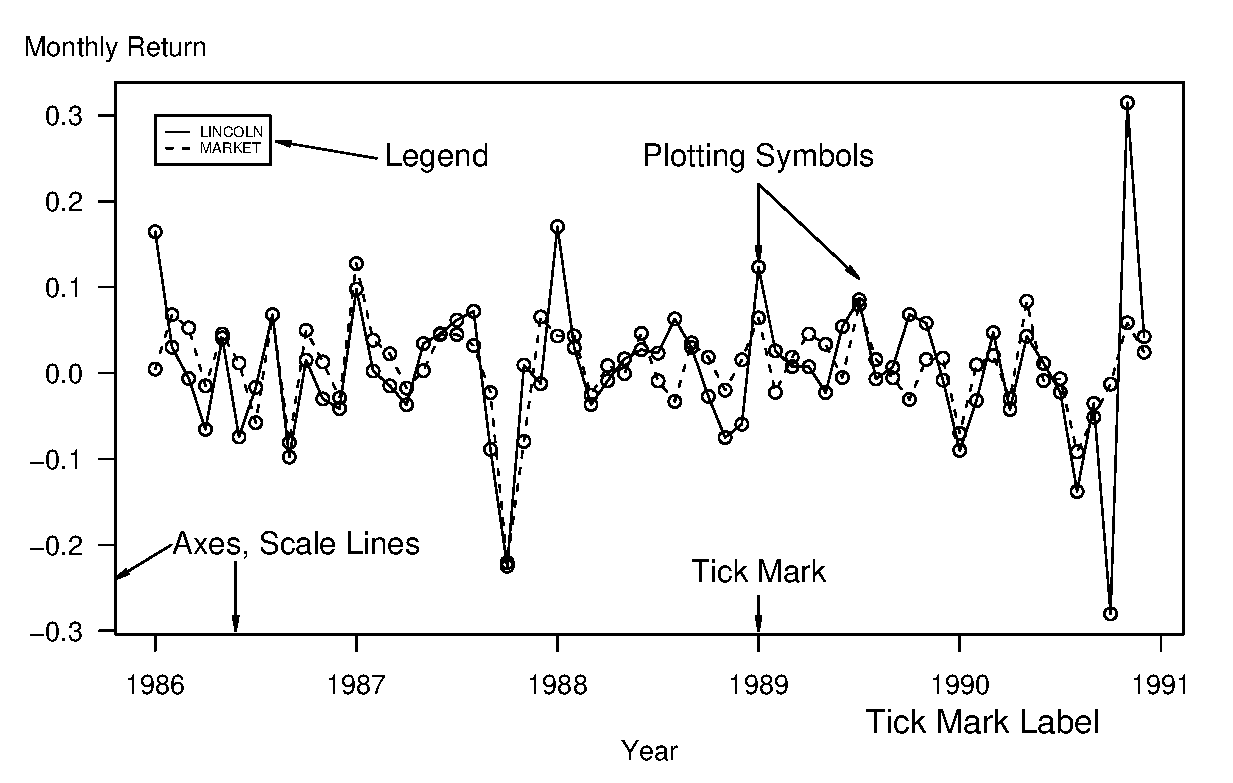
\includegraphics[width=1\textwidth]{Chapter20ReportWriting/F20TimeSeriesPlots.eps}
    \caption{\label{F20:TimeSeriesPlots} \small Time series
plot of returns from the Lincoln National Corporation and the
market. There are 60 monthly returns over the period January, 1986
through December, 1990.}
  \end{center}
\begin{picture}(150,12)
\put (-160,60){\large Title \vector(2,-1){40}}

\end{picture}

\end{figure}




\medskip
\begin{compactenum}[1.]
\item \emph{Title} and \emph{Caption}. As with a table, these provide short descriptions of the
main features of the figure. Long captions may be used to describe
everything that is being graphed, draw attention to the important
features and describe the conclusions to be drawn from the data.
Include the source of the data here or on a separate line
immediately below the graph.

\index{plots!components!title and caption}
\index{plots!components!scale lines and labels}
\index{plots!components!tick marks} \index{plots!components!plotting
symbols} \index{plots!components!legend}

\item \emph{Scale Lines (Axes)} and \emph{Scale Labels}. Choose the scales so that the data fill
up as much of the data region as possible. Do not insist that zero
be included; assume that the viewer will look at the range of the
scales and understand them.
\item \emph{Tick Marks} and \emph{Tick Mark Labels}. Choose the range of the tick marks to include
almost all of the data. Three to ten tick marks are generally
sufficient. When possible put the tick outside of the data region,
so that they do not interfere with the data.

\item \emph{Plotting Symbols}. Use different plotting symbols to encode different levels
of a variable. Plotting symbols should be chosen so that they are
easy to identify, for example, ``O'' for one and ``T'' for two.
However, be sure that plotting symbols are easy to distinguish; for
example, it can be difficult to distinguish ``F'' and ``E''.

\item \emph{Legend (Keys)}. These are small textual displays that help to identify certain
aspects of the data. Do not let these displays interfere with the
data or clutter the graph.
\end{compactenum}
\medskip

As with tables, graphs are separate from the main body of the text
and thus should be self-contained. Especially with long documents,
tables and graphs may contain a separate story line, providing a
look at the main message of the document in a different way than the
main body of the text. Cleveland (1994) and Tufte (1990) provide
several tips to make graphs more ``user-friendly.''

\medskip
\begin{compactenum}[1.]

\item Make lines as thin as possible. Thin lines distract the eye less from the
data when compared to thicker lines. However, make the lines thick
enough so that the image will not degrade under reproduction.

\item Try to use as few lines as possible. Again, several lines distract the eye
from the data, which carries the information. Try to avoid ``grid''
lines, if possible. If you must use grid lines, a light ink, such as
a gray or half tone, is the preferred choice.

\item Spell out words and avoid abbreviations. Rarely is the space saved
worth the potential confusion that the shortened version may cause
the viewer.

\item Use a type that includes both capital and small letters.

\item Place graphs on the same page as the text that discusses the graph.

\item Make words run from left to right, not vertically.

\item Use the substance of the data to suggest the shape and size of the graph.
For time series graphs, make the graph twice as wide as tall. For
scatter plots, make the graph equally wide as tall. If a graph
displays an important message, make the graph large.

\end{compactenum}
\medskip

Of course, for most graphs it will be impossible to follow all these
pieces of advice simultaneously. To illustrate, if we spell out the
scale label on a left hand vertical axis and make it run from left
to right, then we cut into the vertical scale. This forces us to
reduce the size of the graph, perhaps at the expense of reducing the
message.

A graph is a powerful tool for summarizing and presenting numerical
information. Graphs can be used to break up long documents; they can
provoke and maintain reader interest. Further, graphs can reveal
aspects of the data that other methods cannot.


\section{How to Organize}\label{S20:How to Organize}

Writing experts agree that results should be reported in an
organized fashion with some logical flow, although there is no
consensus as to how this goal should be achieved. Every story has a
beginning and an end, usually with an interesting path connecting
the two endpoints. There are many types of paths, or methods of
development, that connect the beginning and the end. For general
technical writing, the method of development may be organized
chronologically, spatially, by order of importance,
general-to-specific or specific-to-general, by cause-and-effect or
any other logical development of the issues. This section presents
one method of organization for statistical report writing that has
achieved desirable results in a number of different circumstances,
including the 10- to 20-page report described previously. This
format, although not appropriate for all situations, serves as a
workable framework on which to base your first statistical report.

The broad outline of the recommended format is:

\medskip

\begin{compactenum}[1.]
\item Title and Abstract
\item Introduction
\item Data Characteristics
\item Model Selection and Interpretation
\item Summary and Concluding Remarks
\item References and Appendix
\end{compactenum}

\medskip

Sections (1) and (2) serve as the preparatory material, designed to
orient the reader. Sections (3) and (4) form the main body of the
report while Sections (5) and (6) are parts of the ending.


\subsection*{Title and Abstract}

If your report is disseminated widely (as you hope), here is some
disappointing news. A vast majority of your intended audience gets
no further than the title and the abstract. Even for readers who
carefully read your report, they will usually carry in their memory
the impressions left by the title and abstract unless they are
experts in the subject that you are reporting on (which most readers
will not be). Choose the title of your report carefully. It should
be concise and to the point. Do not include deadwood (phrases like
\emph{The Study of, An Analysis of}) but do not be too brief, for
example, by using only one word titles. In addition to being
concise, the title should be comprehensible, complete and correct.

\marginparjed{The language of the abstract should be nontechnical.}

The abstract is a one- to two-paragraph summary of your
investigation; 75 to 200 words are reasonable rules of thumb. The
language should be nontechnical as you are trying to reach as broad
an audience as possible. This section should summarize the main
findings of your report. Be sure to respond to such questions as:
What problem was studied? How was it studied? What were the
findings? Because you are summarizing not only your results but also
your report, it is generally most efficient to write this section
last.

\subsection*{Introduction}

As with the general report, the introduction should be partitioned into three
sections: orientation material, key aspects of the report and a plan of the paper.

To begin the orientation material, re-introduce the problem at the
level of technicality that you wish to use in the report. It may or
may not be more technical than the statement of the problem in the
abstract. The introduction sets the pace, or the speed at which new
ideas are introduced, in the report. Throughout the report, be
consistent in the pace. To clearly identify the nature of the
problem, in some instances a short literature review is appropriate.
The literature review cites other reports that provide insights on
related aspects of the same problem. This helps to crystallize the
new features of your report.

As part of the key aspects of the report, identify the source and
nature of the data used in your study. Make sure that the manner in
which your data set can address the stated problem is apparent. Give
an indication of the class of modeling techniques that you intend to
use. Is the purpose behind this model selection clear (for example,
understanding versus forecasting)?

At this point, things can get a bit complex for many readers. It is
a good idea to provide an outline of the remainder of the report at
the close of the introduction. This provides a map to guide the
reader through the complex arguments of the report. Further, many
readers will be interested only in specific aspects of the report
and, with the outline, will be able to ``fast-forward'' to the
sections that interest them most.

\subsection*{Data Characteristics}


\marginparjed{It is also useful to describe the data without
reference to a specific model.}

In a data analysis project, the job is to summarize the data and use
this summary information to make inferences about the state of the
world. Much of this summarization is done through statistics that
are used to estimate model parameters. However, it is also useful to
describe the data without reference to a specific model for at least
two reasons. First, by using basic summary measures of the data, you
can appeal to a larger audience than if you had restricted your
considerations to a specific statistical model. Indeed, with a
carefully constructed graphical summary device, you should be able
to reach virtually any reader who is interested in the subject
material. Conversely, familiarity with statistical models requires a
certain amount of mathematical sophistication and you may or may not
wish to restrict your audience at this stage of the report. Second,
constructing statistics that are immediately connected to specific
models leaves you open to the criticism that your model selection is
incorrect. For most reports, the selection of a model is an
unavoidable juncture in the process of inference but you need not do
it at this relatively early stage of your report.

In the data characteristics section, identify the nature of data.
For example, be sure to identify the component variables, and state
whether the data are longitudinal versus cross-sectional,
observational versus experimental and so forth. Present any basic
summary statistics that would help the reader develop an overall
understanding of the data. It is a good idea to include about two
graphs. Use scatter plots to emphasize primary relationships in
cross-sectional data and time series plots to indicate the most
important longitudinal trends. The graphs, and concomitant summary
statistics, should not only underscore the most important
relationships but may also serve to identify unusual points that are
worthy of special consideration. Carefully choose the statistics and
graphical summaries that you present in this section. Do not
overwhelm the reader at this point with a plethora of numbers. The
details presented in this section should foreshadow the development
of the model in the subsequent section. Other salient features of
the data may appear in the appendix.

\subsection*{Model Selection and Interpretation}

This is the heart and soul of your report. The results reported in
this section generally took the longest to achieve. However, the
length of the section need not be in proportion to the time it took
you to accomplish the analysis. Remember, you are trying to spare
readers the anguish that you went through in arriving at your
conclusions. However, at the same time you want to convince readers
of the thoughtfulness of your recommendations. Here is an outline
for the Model Selection and Interpretation Section that incorporates
the key elements that should appear:

\medskip

\begin{compactenum}[1.]
 \item An outline of the section
 \item A statement of the recommended model
 \item An interpretation of the model, parameter estimates and any broad implications
of the model
 \item The basic justifications of the model
 \item An outline of a thought process that would lead up to this model
 \item A discussion of alternative models.
\end{compactenum}

\medskip

In this section, develop your ideas by discussing the general issues first and
specific details later. Use subsections (1)-(3) to address the broad, general concerns
that a nontechnical manager or client may have. Additional details can
be provided in subsections (4)-(6) to address the concerns of the technically inclined
reader. In this way, the outline is designed to accommodate the needs
of these two types of readers. More details of each subsection are described in
the following.

You are again confronted with the conflicting goals of wanting as
large an audience as possible and yet needing to address the
concerns of technical reviewers. Start this all-important section
with an outline of things to come. That will enable the reader to
pick and choose. Indeed, many readers will wish only to examine your
recommended model and the corresponding interpretations and will
assume that your justifications are reliable. So, after providing
the outline, immediately provide a \emph{statement of the
recommended model} in no uncertain terms. Now, it may not be clear
at all from the data set that your recommended model is superior to
alternative models and, if that is the case, just say so. However,
be sure to state, without ambiguity, what you considered the best.
Do not let the confusion that arises from several competing models
representing the data equally well drift over into your statement of
a model.

The statement of a model is often in statistical terminology, a
language used to express model ideas precisely. Immediately follow
the statement of the recommended model with the concomitant
\emph{interpretations}. The interpretations should be done using
nontechnical language. In addition to discussing the overall form of
the model, the parameter estimates may provide an indication of the
strength of any relationships that you have discovered. Often a
model is easily digested by the reader when discussed in terms of
the resulting implications of a model, such as a confidence or
prediction interval. Although only one aspect of the model, a single
implication may be important to many readers.

It is a good idea to discuss briefly some of the technical
\emph{justifications of the model} in the main body of the report.
This is to convince the reader that you know what you are doing.
Thus, to defend your selection of a model, cite some of the basic
justifications such as \textit{t}-statistics, coefficient of
determination, residual standard deviation, and so forth in the main
body and include more detailed arguments in the appendix. To further
convince the reader that you have seriously thought about the
problem, include a brief description of a \emph{thought process}
that would lead one from the data to your proposed model. Do
\emph{not} describe to the reader all the pitfalls that you
encountered on the way. Describe instead a clean process that ties
the model to the data, with as little fuss as possible.

As mentioned, in data analysis there is rarely if ever a ``right'' answer. To
convince the reader that you have thought about the problem deeply, it is a
good idea to mention \emph{alternative models}. This will show that you considered the
problem from more than one perspective and are aware that careful, thoughtful
individuals may arrive at different conclusions. However, in the end, you
still need to give your recommended model and stand by your recommendation.
You will sharpen your arguments by discussing a close competitor and
comparing it with your recommended model.

\subsection*{Summary and Concluding Remarks}

\marginparjed{This final section may may serve as a springboard for
questions and suggestions about future investigations.}

This section should rehash the results of the report in a concise
fashion, in different words than the abstract. The language may or
may not be more technical than the abstract, depending on the tone
that you set in the introduction. Refer to the key questions posed
when you began the study and tie these to the results. This section
may look back over the analysis and may serve as a springboard for
questions and suggestions about future investigations. Include ideas
that you have about future investigations, keeping in mind costs and
other considerations that may be involved in collecting further
information.

\subsection*{References and Appendix}

The appendix may contain many auxiliary figures and analyses. The reader
will not give the appendix the same level of attention as the main body of the
report. However, the appendix is a useful place to include many crucial details
for the technically inclined reader and important features that are not critical
to the main recommendations of your report. Because the level of technical
content here is generally higher than in the main body of the report, it is important
that each portion of the appendix be clearly identified, especially with
respect to its relation to the main body of the report.



\section{Further Suggestions for Report Writing}

\begin{compactenum}[1.]

\item Be as brief as you can although still include all important details. On
one hand, the key aspects of several regression outputs can often be
summarized in one table. Often a number of graphs can be summarized
in one sentence. On the other hand, recognize the value of a
well-constructed graph or table for conveying important information.

\item Keep your readership in mind when writing your report. Explain what
you now understand about the problem, with little emphasis on how you
happened to get there. Give practical interpretations of results, in language
the client will be comfortable with.

\item Outline, outline. Develop your ideas in a logical, step-by-step fashion. It
is \emph{vital} that there be a logical flow to the report. Start
with a broad outline that specifies the basic layout of the report.
Then make a more detailed outline, listing each issue that you wish
to discuss in each section. You only retain literary freedom by
imposing structure on your reporting.

\item Simplicity, simplicity, simplicity. Emphasize your primary ideas through
simple language. Replace complex words by simpler words if the
meaning remains the same. Avoid the use of cliches and trite
language. Although technical language may be used, avoid the use of
technical jargon or slang. Statistical jargon, such as ``Let $x_1,
x_2, \ldots$ be i.i.d. random variables ...'' is rarely necessary.
Limit the use of Latin phrases (e.g., i.e.) if an English phrase
will suffice (such as, that is).

\item Include important summary tables and graphs in the body of the report.
Label all figures and tables so each is understandable when viewed
alone.

\item Use one or more appendices to provide supporting details. Graphs of secondary
importance, such as residuals plots, and statistical software output,
such as regression fits, can be included in an appendix. Include
enough detail so that another analyst, with access to the data, could replicate
your work. Provide a strong link between the primary ideas that are
described in the main body of the report and the supporting material in
the appendix.
\end{compactenum}


\newpage
\section{Case Study: Swedish Automobile Claims}
\empexjed{SwedishMotorInsurance}\index{datasets!Swedish automobile
claims}


\bigskip
\begin{center}\textbf{Determinants of Swedish Automobile Claims}
\end{center}

\noindent \textbf{Abstract}

\noindent Automobile ratemaking depends on an actuary's ability to
estimate the probability of a claim and, in the event of a claim,
the likely amount. This study examines a classic Swedish data set of
third party automobile insurance claims. Poisson and gamma
regression models were fit to the frequency and severity portions,
respectively. Distance driven by a vehicle, geographic area, recent
driver claims experience and the type of automobile are shown to be
important determinants of claim frequency. \marginparjed{What
problem was studied? How was it studied? What were the findings?}
Only geographic area and automobile type turn out to be important
determinants of claim severity. Although the experience is dated,
the techniques used and the importance of these determinants give
helpful insights into current experience.

\bigskip

\noindent \textbf{Section 1. Introduction}

\noindent Actuaries seek to establish premiums that are fair to
consumers in the sense that each policyholder pays according to his
or her own expected claims. These expected claims are based on
policyholder characteristics that may include age, gender and
driving experience. Motivation for this rating principle is not
entirely altruistic; an actuary understands that rate mispricing can
lead to serious adverse financial consequences for the insuring
company. For example, if rates are too high relative to the
marketplace, then the company is unlikely to gain sufficient market
share. Conversely, if rates are too low relative to actual
experience, then premiums received will be unlikely to cover claims
and related expenses.

\marginparjed{Begin with some orientation material.}

Setting appropriate rates is important in automobile insurance that
indemnifies policyholders and other parties in the event of an
automobile accident. For a short term coverage like automobile
insurance, claims resulting from policies are quickly realized and
the actuary can calibrate the rating formula to actual experience.

For many analysts, data on insurance claims can be difficult to
access. Insurers wish to protect the privacy of their customers and
so do not wish to share data. For some insurers, data are not stored
in an electronic format that is convenient for statistical analyses;
it can be expensive to access data even though it is available to
the insurer. Perhaps most important, insurers are reluctant to
release data to the public because they fear disseminating
proprietary information that will help their competitors in keen
pricing wars.

\marginparjed{When describing the key aspects of the report, include
sources of data.}

Because of this lack of up to date automobile data, this study
examines a classic Swedish data set of third party automobile
insurance claims that occurred in 1977. Third party claims involve
payments to someone other than the policyholder and the insurance
company, typically someone injured as a result of an automobile
accident. Although the experience is dated, the regression
techniques used in this report work equally well with current
experience. Further, the determinants of claims investigated, such
as vehicle use and driver experience, are likely to be important
into today's driving world.

\marginparjed{Provide a plan for the remainder of the paper.}

The outline of the remainder of this report is as follows. In
Section 2, I present the most important characteristics of the data.
To summarize these characteristics, in Section 3 is the discussion
of a model to represent the data. Concluding remarks can be found in
Section 4 and many of the details of the analysis are in the
appendix.

\bigskip
\noindent \textbf{Section 2. Data Characteristics}

\noindent These data were compiled by the Swedish Committee on the
Analysis of Risk Premium in Motor Insurance, summarized in Hallin
and Ingenbleek (1983) and Andrews and Herzberg (1985). The data are
cross-sectional, describing third party automobile insurance claims
for the year 1977.

\marginparjed{Identify the nature of the data.}

The outcomes of interest are the number of claims (the frequency)
and sum of payments (the severity), in Swedish kroners. Outcomes are
based on 5 categories of distance driven by a vehicle, broken down
by 7 geographic zones, 7 categories of recent driver claims
experience (captured by the ``bonus'') and 9 types of automobile.
Even though there are 2,205 potential distance, zone, experience and
type combinations ($5 \times 7 \times 7 \times 9 = 2,205$), only
$n=2,182$ were realized in the 1977 data set. For each combination,
in addition to outcomes of interest, we have available the number of
policyholder years as a measure of exposure. A ``policyholder year''
is the fraction of the year that the policyholder has a contract
with the issuing company. More detailed explanations of these
variables are available in Appendix A2.

\marginparjed{Use selected plots and statistics to emphasize the
primary trends. Do not refer to a statistical model in this
section.}

In this data, there were 113,171 claims from 2,383,170 policyholder
years, for a 4.75\% claims rate. From these claims, a total of
560,790,681 kroners were paid, for an average of 4,955 per claim.
For reference, in June of 1977, a Swedish kroner could be exchanged
for 0.2267 U.S. dollars.

Table \ref{T20:SwedishSumStats} provides more details on the
outcomes of interest. This table is organized by the $n=2,182$
distance, zone, experience and type combinations. For example, the
combination with the largest exposure (127,687.27 policyholder
years) comes from those driving a minimal amount in rural areas of
southern Sweden, having at least six accident free years and driving
a car that is not one of the basic eight types (Kilometres=1,
Zone=4, Bonus=7 and Make=9, see Appendix A2). This combination had
2,894 claims with payments of 15,540,162 kroners. Further, I note
that there were 385 combinations that had zero claims.

\begin{table}[h]
\caption{\label{T20:SwedishSumStats} Swedish Automobile Summary
Statistics}\begin{center}
\begin{tabular}{lrrrrr}
\hline
                     &  & & Standard &  &  \\
Variable & Mean & Median & Deviation & Minimum & Maximum \\
\hline
Policyholder Years &   1,092.20 &      81.53 &   5,661.16 &       0.01 & 127,687.27 \\
    Claims &      51.87 &       5.00 &     201.71 &       0.00 &   3,338.00 \\
   Payments & 257,008&  27,404 & 1,017,283 &       0 & 18,245,026 \\
Average Claim Number&      0.069 &      0.051 &      0.086 &      0.000 &      1.667 \\
 ~~~ (per Policyholder Year)  \\
Average Payment  &   5,206.05 &   4,375.00 &   4,524.56 &      72.00 &  31,442.00 \\
 ~~~ (per Claim) &   \\
\hline \multicolumn{6}{l}{\small \textit{Note:} Distributions are
based on $n=2,182$ distance, zone, experience}\\
\multicolumn{6}{l}{\small ~~~~~~~ and type combinations.}\\
\multicolumn{6}{l}{\textit{Source}: Hallin and Ingenbleek (1983)} \\
\hline
\end{tabular}\end{center}\end{table}


Table \ref{T20:SwedishSumStats} also shows the distribution of the
average claim number per insured. Not surprisingly, the largest
average claim number occurred in a combination where there was only
a single claim with a small number (0.6) of policyholder years.
Because we will be using policyholder years as a weight in our
Section 3 analysis, this type of aberrant behavior will be
automatically down-weighted and so no special techniques are
required to deal with it. For the largest average payment, it turns
out that there are 27 combinations with a single claim of 31,442
(and one combination with two claims of 31,442). This apparently
represents some type of policy limit imposed that we do not have
documentation on. I will ignore this feature in the analysis.


Figure \ref{F20:SPlots} shows the relationships between the outcomes
of interest and exposure bases. For the number of claims, we use
policyholder years as the exposure basis. It is clear that the
number of insurance claims increases with exposure. Further, the
payment amounts increase with the claims number in a very linear
fashion.

\begin{figure}[htp]
  \begin{center}
    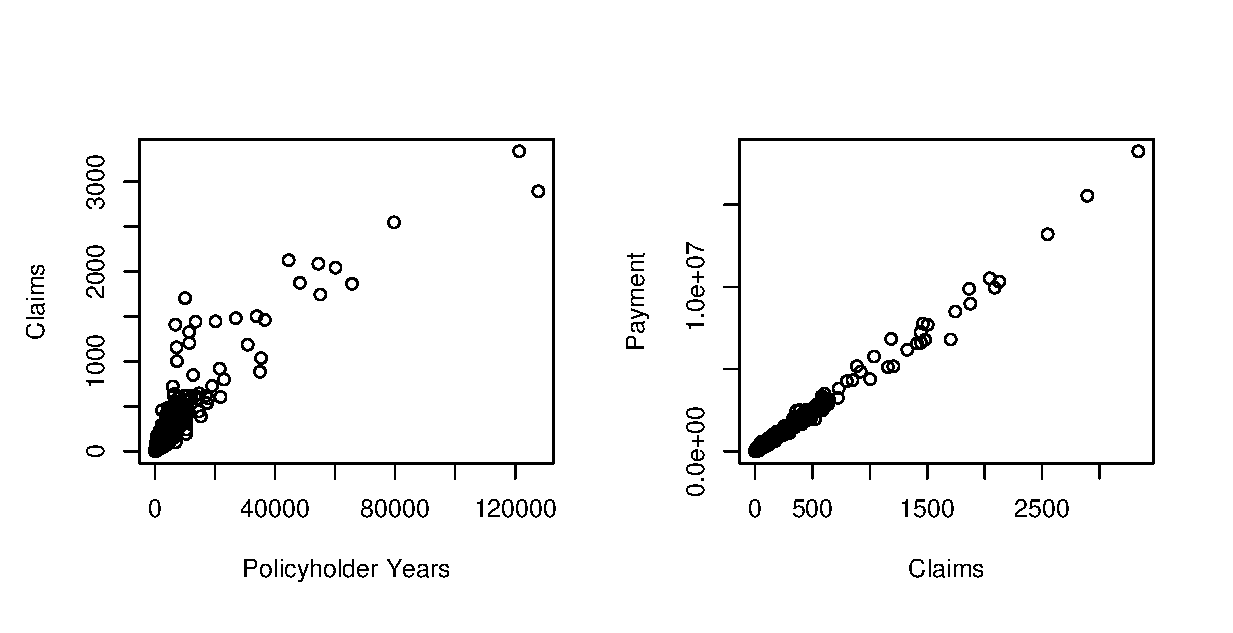
\includegraphics[width=1\textwidth]{Chapter20ReportWriting/F20ScatterPlots.eps}
    \caption{\label{F20:SPlots} \small  Scatter Plots of Claims versus Policyholder Years and Payments versus Claims.}
  \end{center}
\end{figure}


To understand the explanatory variable effects on frequency, Figure
\ref{F20:BoxFreq} presents box plots of the average claim number per
insured versus each rating variable. To visualize the relationships,
three combinations where the average claim exceeds 1.0 have been
omitted. This figure shows lower frequencies associated with lower
driving distances, non-urban locations and higher number of accident
free years. The automobile type also appears to have a strong impact
on claim frequency.


\begin{figure}[htp]
  \begin{center}
    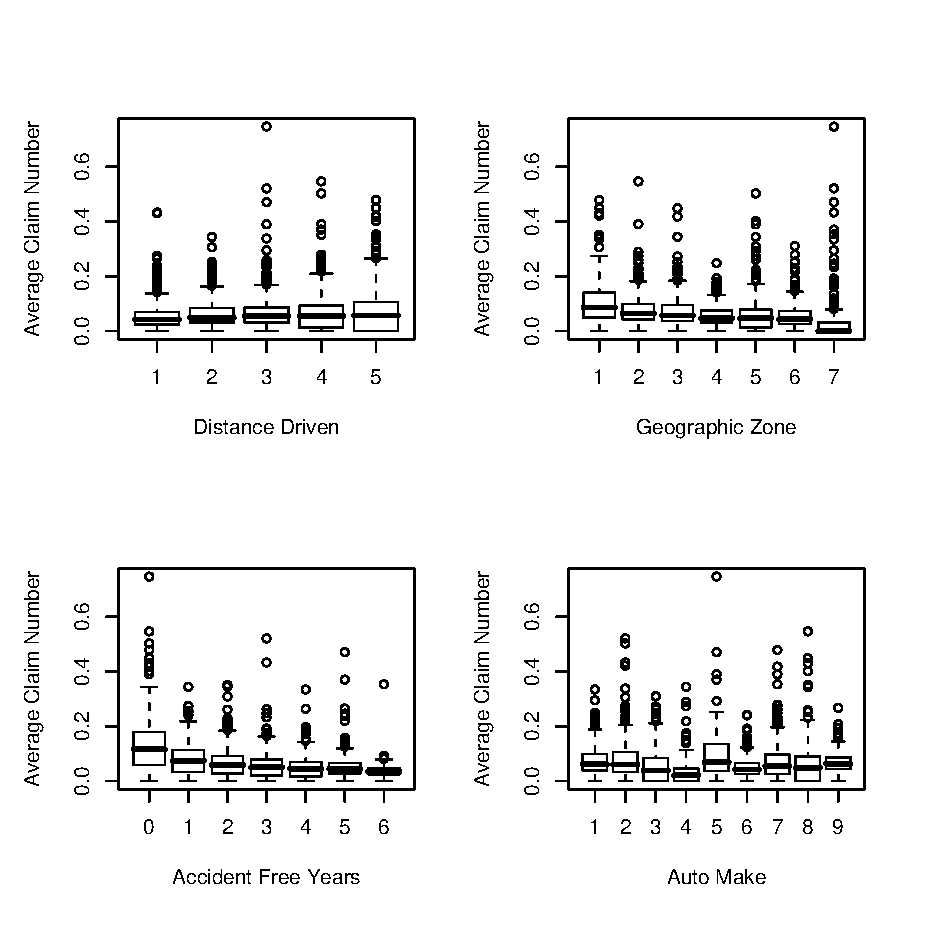
\includegraphics[width=1\textwidth]{Chapter20ReportWriting/F20BoxFREQ.eps}
    \caption{\label{F20:BoxFreq} \small  Box Plots of Frequency by Distance Driven,
    Geographic Zone, Accident Free Years and Make of Automobile.}
  \end{center}
\end{figure}

For severity, Figure \ref{F20:BoxSev} presents box plots of the
average payment per claim versus each rating variable. Here, effects
of the explanatory variables are not as pronounced as with
frequency. The upper right hand panel shows that the average
severity is much smaller for Zone=7. This corresponds to Gotland, a
county and municipality of Sweden that occupies the largest island
in the Baltic Sea. Figure \ref{F20:BoxSev} also suggests some
variation based on the type of automobile.


\begin{figure}[htp]
  \begin{center}
    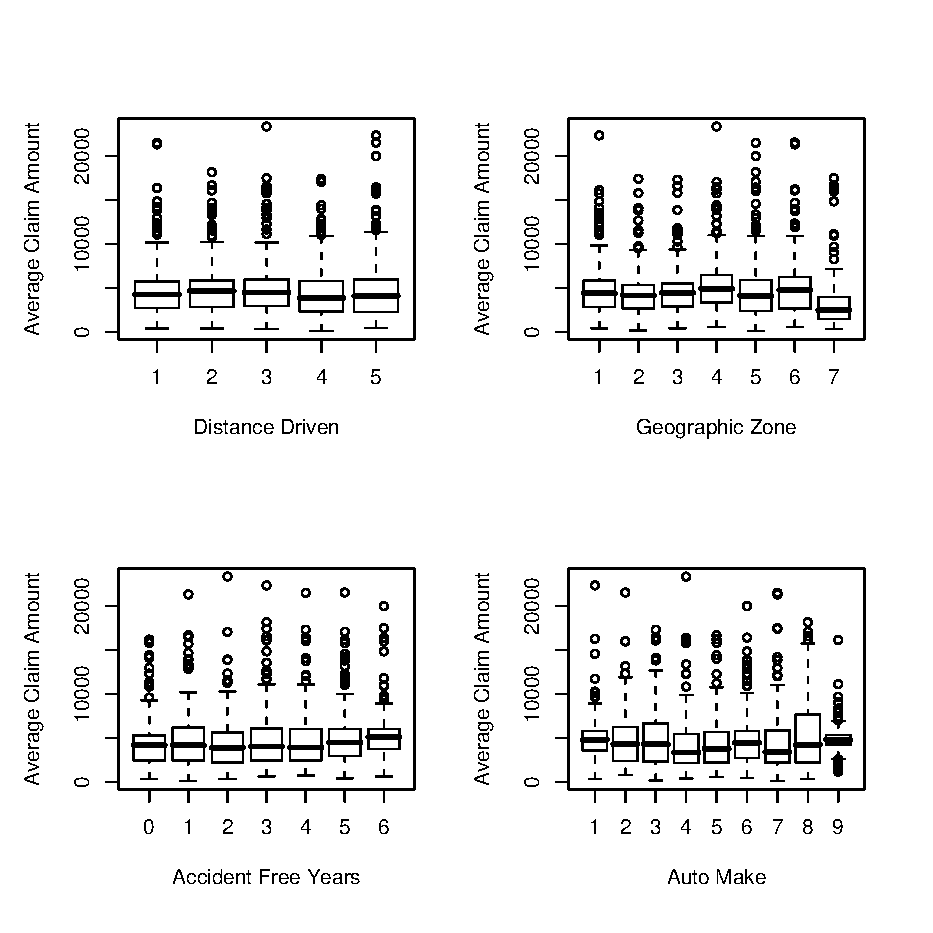
\includegraphics[width=1\textwidth]{Chapter20ReportWriting/F20BoxSEV.eps}
    \caption{\label{F20:BoxSev} \small  Box Plots of Severity by Distance Driven,
    Geographic Zone, Accident Free Years and Make of Automobile.}
  \end{center}
\end{figure}



\newpage
\noindent \textbf{Section 3. Model Selection and Interpretation}

\noindent Section 2 established that there are real patterns between
claims frequency and severity and the rating variables, despite the
great variability in these variables. This section summarizes these
patterns using regression modeling. Following the statement of the
model and its interpretation, this section describes features of the
data that drove the selection of the recommended model.

\marginparjed{Start with a statement of your recommended model.}

As a result of this study, I recommend a Poisson regression model
using a logarithmic link function for the frequency portion. The
systematic component includes the rating factors distance, zone,
experience and type as additive categorical variables as well as an
offset term in logarithmic number of insureds.


\marginparjed{Interpret the model; discuss variables, coefficients
and broad implications of the model}

This model was fit using maximum likelihood, with the coefficients
appearing in Table \ref{T20:PoissonCoeff}; more details appear in
Appendix A4. Here, the base categories correspond to the first level
of each factor. To illustrate, consider a driver living in Stockholm
(Zone=1) who drives between one and fifteen thousand kilometers per
year (Kilometres=2), has had an accident within the last year
(Bonus=1) and driving car type ``Make=6''. Then, from Table
\ref{T20:PoissonCoeff}, the systematic component is $ -1.813 + 0.213
-0.336 = -1.936.$ For a typical policy from this combination, we
would estimate a Poisson number of claims with mean $\exp(-1.936) =
0.144.$ For example, the probability of no claims within a year is
$\exp(-0.144) = 0.866.$ In 1977, there were 354.4 policyholder years
in this combination, for an expected number of claims of $ 354.4
\times 0.144 = 51.03.$ It turned out that there were only 48 claims
in this combination in 1977.

\begin{table}[h]\begin{center}
\caption{\label{T20:PoissonCoeff} Poisson Regression Model Fit}
\begin{tabular}{lrrlrr}
\hline
  Variable & Coefficient &     $t$-ratio &   Variable & Coefficient &     $t$-ratio \\
\hline
Intercept &     -1.813 &    -131.78 & Bonus=2 &     -0.479 &     -39.61 \\
Kilometres=2 &      0.213 &      28.25 & Bonus=3 &     -0.693 &     -51.32 \\
Kilometres=3 &      0.320 &      36.97 & Bonus=4 &     -0.827 &     -56.73 \\
Kilometres=4 &      0.405 &      33.57 & Bonus=5 &     -0.926 &     -66.27 \\
Kilometres=5 &      0.576 &      44.89 & Bonus=6 &     -0.993 &     -85.43 \\
Zone=2 &     -0.238 &     -25.08 & Bonus=7 &     -1.327 &    -152.84 \\
Zone=3 &     -0.386 &     -39.96 & Make=2 &      0.076 &       3.59 \\
Zone=4 &     -0.582 &     -67.24 & Make=3 &     -0.247 &      -9.86 \\
Zone=5 &     -0.326 &     -22.45 & Make=4 &     -0.654 &     -27.02 \\
Zone=6 &     -0.526 &     -44.31 & Make=5 &      0.155 &       7.66 \\
Zone=7 &     -0.731 &     -17.96 & Make=6 &     -0.336 &     -19.31 \\
           &            &            & Make=7 &     -0.056 &      -2.40 \\
           &            &            & Make=8 &     -0.044 &      -1.39 \\
           &            &            & Make=9 &     -0.068 &      -6.84 \\
\hline
\end{tabular}
\end{center}
\end{table}

For the severity portion, I recommend a gamma regression model using
a logarithmic link function. The systematic component consists of
the rating factors zone and type as additive categorical variables
as well as an offset term in logarithmic number of claims. Further,
the square root of the claims number was used as a weighting
variable to give larger weight to those combinations with greater
number of claims.

This model was fit using maximum likelihood, with the coefficients
appearing in Table \ref{T20:GammaCoeff}; more details appear in
Appendix A6. Consider again our illustrative driver living in
Stockholm (Zone=1) who drives between one and fifteen thousand
kilometers per year (Kilometres=2), has had an accident within the
last year (Bonus=1) and driving car type ``Make=6''. For this
person, the systematic component is $ 8.388 + 0.108 = 8.496.$ Thus,
the expected claims under the model are $\exp(8.496) = 4,895.$ For
comparison, the average 1977 payment was 3,467 for this combination
and 4,955 per claim for all combinations.



\begin{table}[h]\begin{center}
\caption{\label{T20:GammaCoeff} Gamma Regression Model Fit}
\begin{tabular}{lrrlrr}
\hline
  Variable & Coefficient &     $t$-ratio &   Variable & Coefficient &     $t$-ratio \\
\hline
 Intercept &      8.388 &      76.72 &     Make=2 &     -0.050 &      -0.44 \\
    Zone=2 &     -0.061 &      -0.64 &     Make=3 &      0.253 &       2.22 \\
    Zone=3 &      0.153 &       1.60 &     Make=4 &      0.049 &       0.43 \\
    Zone=4 &      0.092 &       0.94 &     Make=5 &      0.097 &       0.85 \\
    Zone=5 &      0.197 &       2.12 &     Make=6 &      0.108 &       0.92 \\
    Zone=6 &      0.242 &       2.58 &     Make=7 &     -0.020 &      -0.18 \\
    Zone=7 &      0.106 &       0.98 &     Make=8 &      0.326 &       2.90 \\
           &            &            &     Make=9 &     -0.064 &      -0.42 \\
    Dispersion &  0.483 \\
\hline
\end{tabular}\end{center}
\end{table}
\begin{center}
\textbf{Discussion of the Frequency Model}\end{center}

\marginparjed{What are some of the basic justifications of the
model?}

Both models provided a reasonable fit to the available data. For the
frequency portion, the $t$-ratios in Table \ref{T20:PoissonCoeff}
associated with each coefficient exceed three in absolute value,
indicating strong statistical significance. Moreover, Appendix A5
demonstrates that each categorical factor is strongly statistically
significant.

\marginparjed{Provide strong links between the main body of the
report and the appendix.}

There were no other major patterns between the residuals from the
final fitted model and the explanatory variables. Figure A1 displays
a histogram of the deviance residuals, indicating approximate
normality, a sign that the data are in congruence with model
assumptions.

A number of competing frequency models were considered. Table
\ref{T20:FreqModelComparison} lists two others, a Poisson model
without covariates and a negative binomial model with the same
covariates as the recommended Poisson model. This table shows that
the recommended model is best among these three alternatives, based
on the Pearson goodness of fit statistic and a version weighted by
exposure. Recall that the Pearson fit statistic is of the form $\sum
(O-E)^2/E$, comparing observed ($O$) to data expected under the
model fit ($E$). The weighted version summarizes $\sum w(O-E)^2/E$,
where our weights are policyholder years in units of 100,000. In
each case, we prefer models with smaller statistics. Table
\ref{T20:FreqModelComparison} shows that the recommended model is
the clear choice among the three competitors.


\begin{table}[h]\begin{center}
\caption{\label{T20:FreqModelComparison} Pearson Goodness of Fit for
Three Frequency Models}
\begin{tabular}{lrr}
\hline Model & Pearson & Weighted Pearson \\
\hline
Poisson without Covariates & 44,639 &653.49 \\
Final Poisson Model&  3,003  & 6.41\\
Negative Binomial Model&  3,077 &  9.03\\
\hline
\end{tabular}\end{center}
\end{table}


\marginparjed{Is there a thought process that leads us to conclude
the model is a useful one?}

In developing the final model, the first decision made was to use
the Poisson distribution for counts. This is in accord with accepted
practice and because a histogram of claims numbers (not displayed
here) showed a skewed Poisson-like distribution.

Covariates displayed important features that could affect the
frequency, as shown in Section 2 and Appendix A3.

\marginparjed{A good way to justify your recommended model is to
compare it to one or more alternatives.}

In addition to the Poisson and negative binomial models, I also fit
a quasi-Poisson model with an extra parameter for dispersion.
Although this seemed to be useful, ultimately I chose not to
recommend this variation because the ratemaking goal is to fit
expected values. All rating factors were very statistically
significant with and without the extra dispersion factor and so the
extra parameter added only complexity to the model. Hence, I elected
not to include this term.

\bigskip
\begin{center}
\textbf{Discussion of the Severity Model}\end{center}

For the severity model, the categorical factors zone and make are
statistically significant, as shown in Appendix A7. Although not
displayed here, residuals from this model were well-behaved.
Deviance residuals were approximately normally distributed.
Residuals, when rescaled by the square root of the claims number
were approximately homoscedastic. There were no apparent relations
with explanatory variables.

This complex model was specified after a long examination of the
data. Based on the evident relations between payments and number of
claims in Figure \ref{F20:SPlots}, the first step was to examine the
distribution of payments per claim. This distribution was skewed and
so an attempt to fit logarithmic payments per claim was made. After
fitting explanatory variables to this dependent variable, residuals
from the model fitting were heteroscedastic. These were weighted by
the square root of the claims number and achieved approximate
homoscedasticity. Unfortunately, as seen in Appendix Figure A2, the
fit is still poor in the lower tails of the distribution.

A similar process was then undertaken using the gamma distribution
with a log-link function, with payments as the response and
logarithmic claims number as the offset. Again, I established the
need for the square root of the claims number as a weighting factor.
The process began with all four explanatory variables but distance
and accident free years were dropped due to their lack of
statistical significance. I also created a binary variable ``Safe''
to indicate that a driver had six or more accident free years (based
on my examination of Figure \ref{F20:BoxSev}). However, this turned
out to be not statistically significant and so was not included in
the final model specification.


\bigskip
\noindent \textbf{Section 4. Summary and Concluding Remarks}


\noindent Although insurance claims vary significantly, we have seen
that it is possible to establish important determinants of claims
number and payments. The recommended regression models conclude that
insurance outcomes can be explained in terms of the distance driven
by a vehicle, geographic area, recent driver claims experience and
type of automobile. Separate models were developed for the frequency
and severity of claims. It part, this was motivated by the evidence
that fewer variables seem to influence payment amounts compared to
claims number.

\marginparjed{Rehash the results in a concise fashion. Discuss
shortcomings and potential extensions of the work.}

This study was based on 113,171 claims from 2,383,170 policyholder
years, for a total of 560,790,681 kroners. This is a large data set
that allows us to develop complex statistical models. The grouped
form of the data allows us to work with only $n=2,182$ cells,
relatively small by today's standards. Ungrouped data would have the
advantage of allowing us to consider additional explanatory
variables. One might conjecture about any number of additional
variables that could be included; age, gender and good student
discount are some good candidates. I note that the article by Hallin
and Ingenbleek (1983) considered vehicle age - this variable was not
included in my database because analysts responsible for the data
publication considered to be an insignificant determinant of
insurance claims.

Further, my analysis of data is based on 1977 experience of Swedish
drivers. The lessons learned from this report may or may not
transfer to modern drivers that are closer. Nonetheless, the
techniques explored in this report should be immediately applicable
with the appropriate set of modern experience.




\newpage
\noindent \textbf{Appendix}
\medskip

\begin{center}\textbf{Appendix Table of Contents}\end{center}

\marginparjed{A table of contents, or outline, is useful for long
appendices.}


\begin{compactenum}[{A}1.]
\item References
\item Variable Definitions
\item Basic Summary Statistics for Frequency
\item Final Fitted Frequency Regression Model---R Output
\item Checking Significance of Factors in the Final Fitted Frequency Regression Model --- R Output
\item Final Fitted Severity Regression Model---R Output
\item Checking Significance of Factors in the Final Fitted Severity Regression Model --- R Output
\end{compactenum}

\medskip

\begin{center}
\textbf{A1. References}
\end{center}

\marginparjed{Include references, detailed data analysis and other
materials of lesser importance in the appendices.}

\scalefont{0.9} Andrews, D. F. and A. M. Herzberg (1985). Chapter 68
in: \textit{A Collection from Many Fields for the Student and
Research Worker}, pp. 413-421. Springer, New York.

Hallin, Marc and Jean-Fran\c{c}ois Ingenbleek (1983). The Swedish
automobile portfolio in 1977: A statistical study.
\textit{Scandinavian Actuarial Journal} 1983: 49-64.

\scalefont{1.11111}

\medskip

\begin{center}
\textbf{A2. Variable Definitions}
\end{center}
\begin{table}[h]
\scalefont{0.9}
\begin{tabular}{ll}
\multicolumn{2}{l}{\textbf{TABLE A.1} Variable Definitions}\\
\hline
  Name &Description
  \\ \hline
Kilometres &  Kilometers traveled per year \\
 &   1: $< $1,000 \\
 &  2: 1,000-15,000 \\
 &  3: 15,000-20,000 \\
  & 4: 20,000-25,000 \\
 &   5: $>$ 25,000 \\
\hline
Zone &  Geographic zone \\
 & 1: Stockholm, G\"{o}teborg, Malm\"{o} with surroundings \\
 & 2: Other large cities with surroundings \\
 & 3: Smaller cities with surroundings in southern Sweden \\
 & 4: Rural areas in southern Sweden \\
& 5: Smaller cities with surroundings in northern Sweden \\
& 6: Rural areas in northern Sweden \\
 & 7: Gotland   \\
\hline
 Bonus & No claims bonus. \\
  & ~~~~ Equal to the number of years, plus one, since the last claim.\\
  Make & 1-8 represent eight different common car models.  \\
 & $~~~$ All other models are combined in class 9. \\
Exposure & Amount of policyholder years \\
Claims & Number of claims \\
 Payment & Total value of payments in Swedish kroner
\\ \hline
\end{tabular}
\scalefont{1.1111}
\end{table}


\newpage
\begin{center}
\textbf{A3. Basic Summary Statistics for Frequency}
\end{center}
\scalefont{0.8}

\textbf{TABLE A.2. Averages of Claims per Insured by Rating Factor}

\boxedjed
\begin{alltt}
Kilometre
     1      2      3      4      5
0.0561 0.0651 0.0718 0.0705 0.0827

Zone
     1      2      3      4      5      6      7
0.1036 0.0795 0.0722 0.0575 0.0626 0.0569 0.0504

Bonus
     1      2      3      4      5      6      7
0.1291 0.0792 0.0676 0.0659 0.0550 0.0524 0.0364

Make
     1      2      3      4      5      6      7      8      9
0.0761 0.0802 0.0576 0.0333 0.0919 0.0543 0.0838 0.0729 0.0712
\end{alltt}
\end{boxedminipage}
\scalefont{1.25}


\medskip
\newpage


\begin{center}
 \textbf{A4. Final Fitted Frequency Regression Model --- R Output}
\end{center}
\boxedjed
\scalefont{0.8}
\begin{alltt}


Call: glm(formula = Claims ~ factor(Kilometres) + factor(Zone) +
factor(Bonus) +
    factor(Make), family = poisson(link = log), offset = log(Insured))

Deviance Residuals:
   Min      1Q  Median      3Q     Max
-6.985  -0.863  -0.172   0.600   6.401

Coefficients:
                    Estimate Std. Error z value Pr(>|z|)
(Intercept)         -1.81284    0.01376 -131.78  < 2e-16 ***
factor(Kilometres)2  0.21259    0.00752   28.25  < 2e-16 ***
factor(Kilometres)3  0.32023    0.00866   36.97  < 2e-16 ***
factor(Kilometres)4  0.40466    0.01205   33.57  < 2e-16 ***
factor(Kilometres)5  0.57595    0.01283   44.89  < 2e-16 ***
factor(Zone)2       -0.23817    0.00950  -25.08  < 2e-16 ***
factor(Zone)3       -0.38639    0.00967  -39.96  < 2e-16 ***
factor(Zone)4       -0.58190    0.00865  -67.24  < 2e-16 ***
factor(Zone)5       -0.32613    0.01453  -22.45  < 2e-16 ***
factor(Zone)6       -0.52623    0.01188  -44.31  < 2e-16 ***
factor(Zone)7       -0.73100    0.04070  -17.96  < 2e-16 ***
factor(Bonus)2      -0.47899    0.01209  -39.61  < 2e-16 ***
factor(Bonus)3      -0.69317    0.01351  -51.32  < 2e-16 ***
factor(Bonus)4      -0.82740    0.01458  -56.73  < 2e-16 ***
factor(Bonus)5      -0.92563    0.01397  -66.27  < 2e-16 ***
factor(Bonus)6      -0.99346    0.01163  -85.43  < 2e-16 ***
factor(Bonus)7      -1.32741    0.00868 -152.84  < 2e-16 ***
factor(Make)2        0.07624    0.02124    3.59  0.00033 ***
factor(Make)3       -0.24741    0.02509   -9.86  < 2e-16 ***
factor(Make)4       -0.65352    0.02419  -27.02  < 2e-16 ***
factor(Make)5        0.15492    0.02023    7.66  1.9e-14 ***
factor(Make)6       -0.33558    0.01738  -19.31  < 2e-16 ***
factor(Make)7       -0.05594    0.02334   -2.40  0.01655 *
factor(Make)8       -0.04393    0.03160   -1.39  0.16449
factor(Make)9       -0.06805    0.00996   -6.84  8.2e-12 ***
---
Signif. codes:  0 �***� 0.001 �**� 0.01 �*� 0.05 �.� 0.1 � � 1

(Dispersion parameter for poisson family taken to be 1)

    Null deviance: 34070.6  on 2181  degrees of freedom
Residual deviance:  2966.1  on 2157  degrees of freedom AIC: 10654
\end{alltt}
\scalefont{1.25}
\end{boxedminipage}

\newpage



\begin{center}
 \textbf{A5. Checking Significance of Factors in the Final Fitted Frequency Regression Model --- R Output}
\end{center}
\boxedjed \scalefont{0.8}
\begin{alltt}
Analysis of Deviance Table

Terms added sequentially (first to last)
                     Df Deviance Resid. Df Resid. Dev P(>|Chi|)
NULL                                  2181      34071
factor(Kilometres)    4     1476      2177      32594  2.0e-318
factor(Zone)          6     6097      2171      26498         0
factor(Bonus)         6    22041      2165       4457         0
factor(Make)          8     1491      2157       2966  1.4e-316
\end{alltt}
\scalefont{1.25}
\end{boxedminipage}



\begin{figure}[htp]
  \begin{center}
    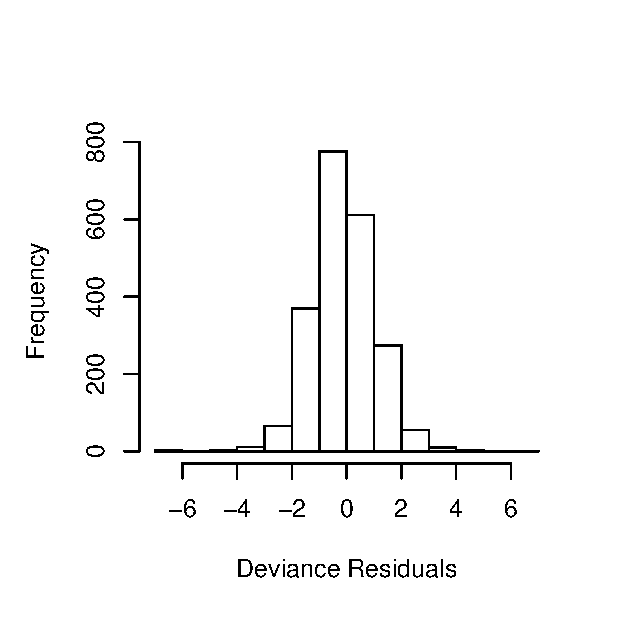
\includegraphics[width=.6\textwidth]{Chapter20ReportWriting/F20Resids.eps}
   \end{center}
  \begin{center}
   \small Figure A1. Histogram of deviance residuals from the
final frequency model
  \end{center}
\end{figure}

\newpage


\begin{center}
 \textbf{A6. Final Fitted Severity Regression Model --- R Output}
\end{center}
\boxedjed \scalefont{0.8}
\begin{alltt}
Call:
glm(formula = Payment ~ factor(Zone) + factor(Make), family = Gamma(link = log),
    weights = Weight, offset = log(Claims))

Deviance Residuals:
     Min        1Q    Median        3Q       Max
-2.56968  -0.39928  -0.06305   0.07179   2.81822

Coefficients:
              Estimate Std. Error t value Pr(>|t|)
(Intercept)    8.38767    0.10933  76.722  < 2e-16 ***
factor(Zone)2 -0.06099    0.09515  -0.641  0.52156
factor(Zone)3  0.15290    0.09573   1.597  0.11041
factor(Zone)4  0.09223    0.09781   0.943  0.34583
factor(Zone)5  0.19729    0.09313   2.119  0.03427 *
factor(Zone)6  0.24205    0.09377   2.581  0.00992 **
factor(Zone)7  0.10566    0.10804   0.978  0.32825
factor(Make)2 -0.04963    0.11306  -0.439  0.66071
factor(Make)3  0.25309    0.11404   2.219  0.02660 *
factor(Make)4  0.04948    0.11634   0.425  0.67067
factor(Make)5  0.09725    0.11419   0.852  0.39454
factor(Make)6  0.10781    0.11658   0.925  0.35517
factor(Make)7 -0.02040    0.11313  -0.180  0.85692
factor(Make)8  0.32623    0.11247   2.900  0.00377 **
factor(Make)9 -0.06377    0.15061  -0.423  0.67205
---
Signif. codes:  0 �***� 0.001 �**� 0.01 �*� 0.05 �.� 0.1 � � 1

(Dispersion parameter for Gamma family taken to be 0.4830309)

    Null deviance: 617.32  on 1796  degrees of freedom
Residual deviance: 596.79  on 1782  degrees of freedom
AIC: 16082
\end{alltt}
\scalefont{1.25}
\end{boxedminipage}

\bigskip

\begin{center}
 \textbf{A7. Checking Significance of Factors in the Final Fitted Severity Regression Model --- R Output}
\end{center}
\boxedjed \scalefont{0.8}
\begin{alltt}
Analysis of Deviance Table

Terms added sequentially (first to last)

               Df Deviance Resid. Df Resid. Dev P(>|Chi|)
NULL                            1796     617.32
factor(Zone)    6     8.06      1790     609.26      0.01
factor(Make)    8    12.47      1782     596.79  0.001130

\end{alltt}
\scalefont{1.25}
\end{boxedminipage}

\begin{figure}[htp]
  \begin{center}
    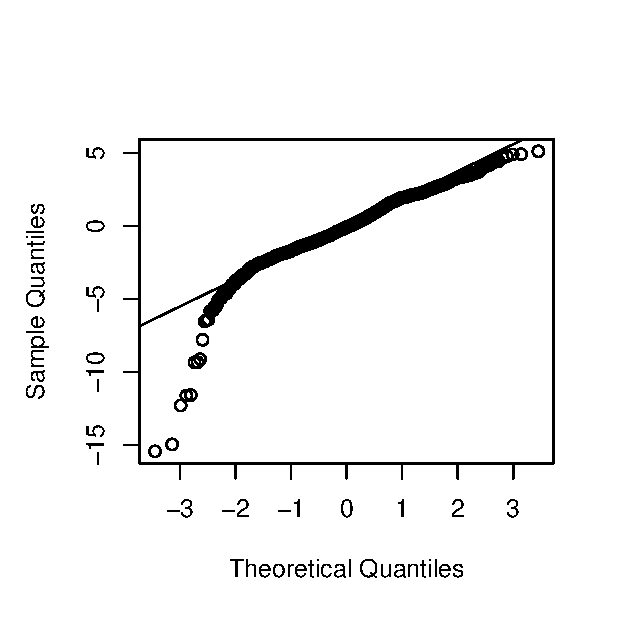
\includegraphics[width=.6\textwidth]{Chapter20ReportWriting/F20QQplot.eps}
   \caption{\small Figure A2. $qq$ Plot of Weighted Residuals from a
   Lognormal Model. The dependent variable is average severity per claim.
    Weights are the square root of the number
   of claims. The poor fit in the tails suggests using an
   alternative to the lognormal model.}
  \end{center}
\end{figure}


\newpage

\section{Further Reading and References}

You can find further discussion of guidelines for presenting within
text data in \emph{The Chicago Manual of Style}, a well-known
reference for preparing and editing written copy.

You can find further discussion of guidelines for presenting tabular
data in Ehrenberg (1977) and Tufte (1983).

Miller (2005) is a book length introduction to writing statistical
reports with an emphasis on regression methods.

\bigskip

\textbf{Chapter References}

\begin{multicols}{2}

\scalefont{0.9}

\emph{The Chicago Manual of Style} (1993). The University of Chicago
Press, 14th ed. Chicago, Ill.

Cleveland, William S. (1994). \emph{The Elements of Graphing Data}.
Monterey, Calif.: Wadsworth.

Ehrenberg, A.S.C. (1977). Rudiments of numeracy. \emph{Journal of
the Royal Statistical Society A} 140:277�97.

Miller, Jane E. (2005). \emph{The Chicago Guide to Writing about
Multivariate Analysis}. The University of Chicago Press, Chicago,
Ill.

Tufte, Edward R. (1983). \emph{The Visual Display of Quantitative
Information}. Graphics Press, Cheshire, Connecticut.

Tufte, Edward R. (1990). \emph{Envisioning Information}. Graphics
Press, Cheshire, Connecticut.


\scalefont{1.1111}

\end{multicols}

\section{Exercises}

\begin{exercises}

\scalefont{0.90}

\empexjed{CeoCompensation}\index{datasets!CEO compensation}


\item Determinants of CEO Compensation. Chief executive officer (CEO) compensation varies
significantly from firm to firm. For this exercise, you will report
on a sample of firms from a survey by \emph{Forbes Magazine} to
establish important patterns in the compensation of CEOs.
Specifically, introduce a regression model that explains CEO
salaries in terms of the firm's sales and the CEO's length of
experience, education level and ownership stake in the firm. Among
other things, this model should show that larger firms tend to pay
CEOs more and, somewhat surprisingly, that CEOs with a higher
educational levels earn less than otherwise comparable CEOs. In
addition to establishing important influences on CEO compensation,
this model should be used to predict CEO compensation for salary
negotiation purposes.


\scalefont{1.1111}

\end{exercises}
